\section{RMS}
Root-Mean-Square (RMS)
The root mean square value is as John bird tells in Engineering Mathematics \cite{Bird2007
} “ the square root of the mean value of the squared values of the quantity over an interval “
One of the principal applications of RMS is with alternating current a.c. and voltage v. The a.c is defined as a current with a heating effect which resemples the direct current. \cite{Bird2007}
\\
For a pure sinewave the RMS value is 0.707 * the peak value
\\
To find the RMS three mathematical operations are used.
(1)	Square the values of the amplitude
(2)	Take the mean of the results from (1)
(3)	Take the square root of the results from (2)
\begin{equation}\label{eq:RMS formular}
RMSy = \frac{1}{N-1}\sum_{u=0}^{N-1}|y[u]|^2
\end{equation}
\\

\\
This is how r.m.s. was used in matlab
\begin{figure}
\begin{center}
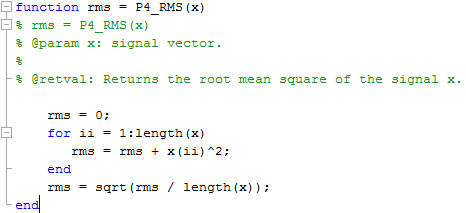
\includegraphics[height=5cm]{fig/RMS_matlabCode.png}
\caption{RMS}
\end{center}
\end{figure}

source1= 2007, john bird, Elsevier, Engineering Mathematics